\documentclass[totpages,helvetica,openbib,italian]{europecv}
\usepackage[T1]{fontenc}
\usepackage{graphicx}
\usepackage[a4paper,top=1.27cm,left=1cm,right=1cm,bottom=2cm]{geometry}
\usepackage[italian]{babel}
\usepackage{bibentry}
\usepackage{url}
\usepackage{enumitem}
\setlist{nolistsep}

\ecvname{Diego Russo}
\ecvaddress{Via G. Garibaldi 40, 05021, Acquasparta (TR), Italia}
\ecvtelephone[+39 334 5873886]{+39 0744 930614}
\ecvemail{\url{me@diegor.it} - (gtalk, MSN)}
\ecvhomepage{\url{http://www.diegor.it}}
\ecvnationality{Italiana}
\ecvdateofbirth{30 aprile 1983}
\ecvgender{Maschio}
\ecvbeforepicture{\raggedleft}
\ecvpicture[width=3cm]{../images/diegor.jpg}
\ecvafterpicture{\ecvspace{-3cm}} 
\ecvfootnote{Per ulteriori informazioni: \url{http://europass.cedefop.eu.int}\\
\textcopyright~European Communities, 2003.}

\begin{document}
    \begin{center}
        \hspace{1pt}
        \vspace{2cm}
    
        {\scshape \textbf{\Huge Diego Russo}}
    
        \vspace{1cm}
    
        {\scshape \textbf{\Large \underline{Curriculum Vitae}}}
    
        \vspace{0.25cm}
    
        {\large aggiornato a \emph{\textbf{Gennaio 2011}}}
        
        \vspace{2cm}
        
        \begin{figure}[htbp] 
            \begin{center} 
                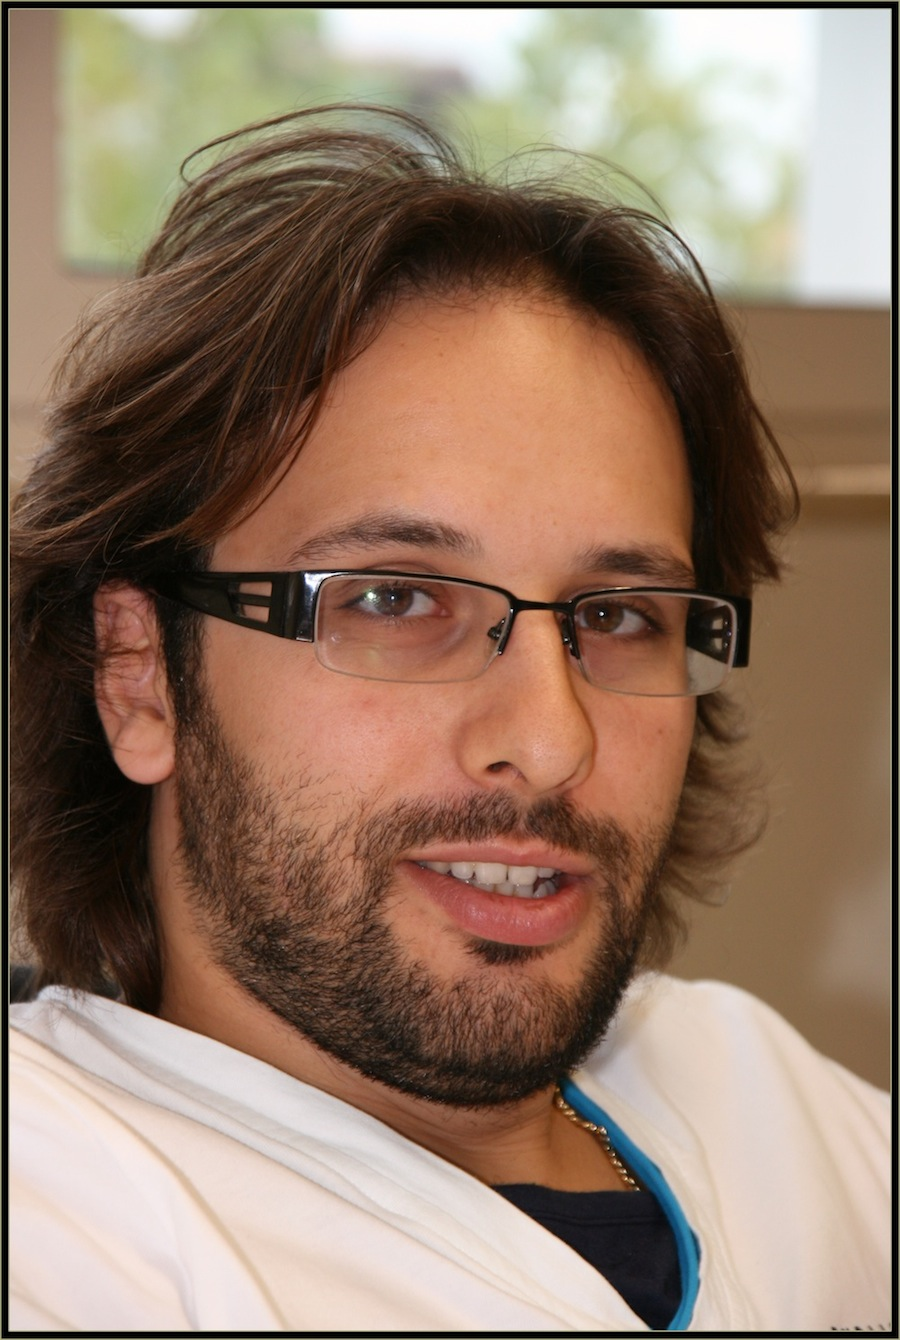
\includegraphics[width=10cm]{../images/io.jpg}
            \end{center} 
        \end{figure}
        
    \end{center}
\pagebreak
\selectlanguage{italian}

\begin{europecv}
\ecvpersonalinfo[5pt]

\ecvitem{\large\textbf{Impiego ricercato/ Settore di competenza}}{\large\textbf{Ricerco posizione in cui possa esprimere la mia passione per la programmazione e la tecnologia. Programmo maggiormente in Python/Django usando quotidianamente Linux e OSX. Aperto ad impieghi che mi diano la possibilit\'a di crescere professionalmente e personalmente.}}

\ecvsection{Esperienza professionale}

\ecvitem{Date}{\textbf{Da dicembre 2006 ad agosto 2008 e da settembre 2009 a giugno 2011}}
\ecvitem{Lavoro o posizione ricoperti}{Programmatore \textbf{Python/Django}}
\ecvitem{Principali attivit\'a e responsabilit\'a}{Lavorando in un team, ho sviluppato un'applicazione gestionale per il comune di Bettona utilizzando Django, Python, PostgreSQL, Linux, Apache, per \textbf{l'informatizzazione dei servizi}, per la gestione delle anagrafiche nonch\'e delle pratiche edilizie ed urbanistiche e del calcolo della tassa ICI con aggiornamenti dei dati catastali. Inoltre ho creato un'avanzata interfaccia web per la presentazione di proposte di pratiche, conferenza dei servizi on-line, integrazione di procedimenti, visione di mappe catastali in \textbf{DXF} e produzione di stampe personalizzate ed automatizzate.

Durante il progetto ho utilizzato controlli di versione del software (SVN/GIT), con relativa interfaccia web (trac) per la gestione dei ticket.}
\ecvitem{Nome e indirizzo del datore di lavoro}{Consorzio Miles - Servizi Integrati, CF 04881101002, Via Rocca di Papa 21, Roma, \url{http://www.consorzio-miles.com/arianna/}}
\ecvitem[10pt]{Tipo di attivit\'a o settore}{Servizi integrati per la pubblica amministrazione}

\ecvitem{Date}{\textbf{Dal 26 aprile 2008 al 15 febbraio 2011}}
\ecvitem{Lavoro o posizione ricoperti}{Programmatore e sistemista nel reparto \textbf{''Ricerca e Sviluppo''}}
\ecvitem{Principali attivit\'a e responsabilit\'a}{Lavorando in un team di ricerca e sviluppo per la creazione di un prodotto innovativo ed unico nel mercato delle comunicazioni senza fili (WiFi), ho lavorato in un primo periodo su \textbf{dispositivi embedded} (ubnt, alix, pcengines) personalizzando fortemente il sistema operativo (ubnt, openwrt) ed i software per gestire l'autenticazione (hostapd, wpa-supplicant). Dopo questa prima fase mi sono concentrato sullo sviluppo di software per il \emph{flashing} di tali dispositivi e per la produzione su larga scala.

Abbiamo inoltre sviluppato una soluzione completa per la gestione di \textbf{un sistema di hotspot}: mi sono occupato dello sviluppo lato server in modo da gestire autenticazioni, log delle sessioni, registrazioni, gestione dei segnali dai nodi, integrazione con i nostri gestionali, pagamenti con carta di credito ed autenticazione tramite SMS, il tutto in regola con la normativa Pisanu.
Come ultimo incarico ho creato un software per il monitoring della rete. Questo tratta di un'applicazione \textbf{stand-alone in PyQT}, utilizzando delle API interne basate su Django.

Le tecnologie utilizzate sono per la maggiore Python/Django con database PostgreSQL su sistemi Debian virtualizzati su XEN.}
\ecvitem{Nome e indirizzo del datore di lavoro}{Forinicom srl, Via del Popolo, 9 Bastia Umbra, 06083, 0758001868, \url{http://www.forinicom.it}}
\ecvitem[10pt]{Tipo di attivit\'a o settore}{Telecomunicazioni}

\ecvitem{Date}{\textbf{Da novembre 2010 a gennaio 2011}}
\ecvitem{Lavoro o posizione ricoperti}{Programmatore \textbf{Python/Django}}
\ecvitem{Principali attivit\'a e responsabilit\'a}{Completamento di una \textbf{WebTV per adulti} interamente sviluppato in Python/Django con database PostgreSQL su piattaforma Linux/Apache e backend di streaming in Red5. Il lavoro \'e interamente gestito in autonomia utilizzando GIT come software di revisione del software.}
\ecvitem{Nome e indirizzo del datore di lavoro}{Exion Sagl - Via Cantonale 2b - 6928 Manno, Switzerland, , \url{http://www.exion.ch/}}
\ecvitem[10pt]{Tipo di attivit\'a o settore}{Soluzioni informatiche}

\ecvitem{Date}{\textbf{Da ottobre 2010 a gennaio 2011}}
\ecvitem{Lavoro o posizione ricoperti}{Programmatore \textbf{Python/Pylons}}
\ecvitem{Principali attivit\'a e responsabilit\'a}{La collaborazione prevede implementazioni di nuove funzionalit\'a, correzione di bug, modifiche strutturali al sito della Sauce Labs. Il coordinamento del lavoro avviene da remoto. Il portale \'e scritto in Python/Pylons utilizzando \url{github.com} come piattaforma di revisione del codice.}
\ecvitem{Nome e indirizzo del datore di lavoro}{Sauce Labs Inc - 500 Third St., San Francisco, CA 94107 USA, \url{http://saucelabs.com/}}
\ecvitem[10pt]{Tipo di attivit\'a o settore}{Cross Browser Testing in the Cloud}

\ecvitem{Date}{\textbf{Dal 30 luglio 2006 al 30 dicembre 2006}}
\ecvitem{Lavoro o posizione ricoperti}{Tesista: Wireless Broadband Network - progetto \textbf{WeConnect}}
\ecvitem{Principali attivit\'a e responsabilit\'a}{Il lavoro di tesi consisteva nello sviluppare una rete WiFi in grado di coprire zone in \textbf{digital-divide}. Grazie a questo progetto ho acquisito ampia conoscenza delle reti wireless, della normativa che ne regola il funzionamento, del sistema operativo RouterOS (\url{www.mikrotik.com}), del protocollo AAA e del server FreeRADIUS. Infine ho amministrato server per l'erogazione di vari servizi di rete: mail (Postfix), server web (Apache), DNS (pdns), firewall (iptables), database (PostgreSQL), hotspot (Chillispot), OS Debian, Voyage (OS per sistemi embedded, basata su Debian).}
\ecvitem{Nome e indirizzo del datore di lavoro}{WEDOIT s.a.s. - Via Protomartiri Francescani,26 - 06088 Assisi (PG), \url{http://www.wedoit.us}}
\ecvitem[10pt]{Tipo di attivit\'a o settore}{Soluzioni informatiche}

\ecvitem{Date}{\textbf{Dal 14 novembre 2005 al 30 maggio 2006}}
\ecvitem{Lavoro o posizione ricoperti}{Stagista - \textbf{S.E.O. Search Engine Optimization}}
\ecvitem{Principali attivit\'a e responsabilit\'a}{Lavorando in un team ho acquisito conoscenze di S.E.O. e dei suoi meccanismi. Lo stage prevedeva l'ottimizzazione S.E.O. di un insieme di siti utilizzando tecniche di \emph{pageranking} e \emph{link popularity}. Inoltre mi sono occupato dell'amministrazione di un server virtuale (basato su Debian) e dello sviluppo di applicazione in Python e PHP orientate al S.E.O.}
\ecvitem{Nome e indirizzo del datore di lavoro}{WEDOIT s.a.s. - Via Protomartiri Francescani,26 - 06088 Assisi (PG), \url{http://www.wedoit.us}}
\ecvitem[10pt]{Tipo di attivit\'a o settore}{Soluzioni informatiche}

\ecvitem{Date}{\textbf{marzo 2002}}
\ecvitem{Lavoro o posizione ricoperti}{Stagista abbinato al progetto IFS, Impresa Formativa Simulata}
\ecvitem{Principali attivit\'a e responsabilit\'a}{Durante lo stage ho gestito della rete interna dell'impresa}
\ecvitem{Nome e indirizzo del datore di lavoro}{IOSA CARLO S.r.l. - 05100 TERNI - Via Pallotta n. 7 - Tel. (0744) 2460 - Fax (0744) 246035 - P.IVA 00072550551 - \url{http://www.iosacarlo.com} - \url{iosacarlo@iosacarlo.com}}
\ecvitem[10pt]{Tipo di attivit\'a o settore}{Impresa smaltimento rifiuti}

\ecvsection{Istruzione e formazione}

\ecvitem{Date}{\textbf{Da ottobre 2008 a oggi}}
\ecvitem{Titolo della qualifica rilasciata}{Iscritto alla specializzazione di Informatica, indirizzo di \textbf{''Sicurezza Informatica''}}
\ecvitem{Principali tematiche/competenze professionali possedute}{Sostenuti i seguenti esami con relativa votazione:\begin{itemize}
    \item Simulazione: 30 e lode
    \item Programmazione Avanzata: 30 e lode
    \item Sistemi operativi avanzati: 30 e lode
    \item Laboratorio di Sistemi operativi avanzati: 30 e lode
\end{itemize}}
\ecvitem{Nome e tipo d'organizzazione erogatrice dell'istruzione e formazione}{Universit\'a degli studi di Perugia, Dipartimento di Informatica, \url{http://informatica.unipg.it}}

\ecvitem{Date}{\textbf{maggio 2010}}
\ecvitem{Titolo della qualifica rilasciata}{\textbf{Diploma de Español como Lengua Extranjera} (DELE) - Diploma di Spagnolo come lingua straniera}
\ecvitem{Principali tematiche/competenze professionali possedute}{I livelli da me raggiunti in questo corso sono:
\begin{itemize}
    \item comprensione di lettura ed espressione scritta: 32,5/35,0 punti
    \item grammatica e vocabolario: 17,33/20 punti
    \item comprensione ed espressione orale: 44,32/45 punti
\end{itemize}}
\ecvitem{Nome e tipo d'organizzazione erogatrice dell'istruzione e formazione}{Instituto Cervantes, C/ Alcal\'a 49, E-28014 Madrid (Spagna), \url{http://www.cervantes.es}}
\ecvitem[10pt]{Livello nella classificazione nazionale o internazionale}{\textbf{Livello B1}\footnote{Valutazione in accordo con l'''Instituto Cervantes de Madrid''}}

\ecvitem{Date}{\textbf{Dal 14 ottobre 2009 ad 26 maggio 2010}}
\ecvitem{Titolo della qualifica rilasciata}{Attestato di frequenza di 42/50 ore del 3$^\circ$ e di 44/50 ore del 4$^\circ$ modulo di lingua spagnola}
\ecvitem{Principali tematiche/competenze professionali possedute}{I livelli da me raggiunti in questo corso sono:
\begin{itemize}
    \item capire gli elementi principali in un discorso chiaro in lingua standard su argomenti familiari
    \item riuscire a descrivere esperienze ed avvenimenti, motivare e spiegare progetti
    \item affrontare molte delle situazioni che si possono presentare viaggiando in una zona dove si parla la lingua
    \item comprendere frasi ed espressioni di uso frequente relativi ad ambiti di immediata rilevanza
    \item saper descrivere in termini semplici aspetti della propria storia e delle proprie esperienze
    \item saper parlare dell'ambiente circostante e saper esprimere bisogni, intenzioni e previsioni
\end{itemize}}
\ecvitem{Nome e tipo d'organizzazione erogatrice dell'istruzione e formazione}{Istituto comprensivo ''Volumnio'' Ponte San Giovanni - Perugia}

\ecvitem{Date}{\textbf{Da agosto 2009 a marzo 2010}}
\ecvitem{Titolo della qualifica rilasciata}{Pubblicazione del paper \textbf{''The AES implentation based on OpenCL for multi/many core architecture''}}
\ecvitem{Principali tematiche/competenze professionali possedute}{Preparazione e pubblicazione del paper ''The AES implentation based on OpenCL for multi/many core architecture'' per l'annuale conferenza ICCSA 2010 (\url{www.iccsa.org}) alla Sangyo University, Fukuoka in Giappone. Il paper tratta di un' implementazione di AES eseguito su core GPU NVIDIA/ATI.}
\ecvitem{Nome e tipo d'organizzazione erogatrice dell'istruzione e formazione}{Universit\'a degli studi di Perugia, Dipartimento di Informatica}

\ecvitem{Date}{\textbf{Da febbraio 2007 a luglio 2007}}
\ecvitem{Titolo della qualifica rilasciata}{Patente di operatore di stazione di \textbf{radioamatore di classe A}}
\ecvitem{Principali tematiche/competenze professionali possedute}{Durante il corso per aspiranti radioamatori ho acquisito ottime conoscenze di radiotecnica, apparecchiature radio e loro funzionamento. Inoltre non sono mancati cenni di fisica e chimica (magnetismo, elettromagnetismo)}
\ecvitem{Nome e tipo d'organizzazione erogatrice dell'istruzione e formazione}{C.I.S.A.R. Sezione di Foligno}
\ecvitem[10pt]{Livello nella classificazione nazionale o internazionale}{IDONEO, Nominativo internazionale \textbf{IZ0OVB}}

\ecvitem{Date}{\textbf{Dal 19 marzo 2007 al 23 marzo 2007}}
\ecvitem{Titolo della qualifica rilasciata}{Attestato di partecipazione al corso di \textbf{lingua spagnola}}
\ecvitem{Principali tematiche/competenze professionali possedute}{Durante il periodo trascorso a Madrid, in questa scuola ho approfondito conoscenze aggiuntive riguardo la grammatica di base e la cultura generale spagnola.}
\ecvitem{Nome e tipo d'organizzazione erogatrice dell'istruzione e formazione}{Inhispania Intlance S.L / CIF:B83744847, Montera 10-12, 1-1. 28013, Madrid (Spagna)}
\ecvitem[10pt]{Livello nella classificazione nazionale o internazionale}{\textbf{Livello A2}\footnote{Valutazione in accordo con il ''Common European Framework of Reference for Languages''}}

\ecvitem{Date}{\textbf{01-02-03 dicembre 2006}}
\ecvitem{Titolo della qualifica rilasciata}{Attestato di partecipazione al corso sulle \textbf{certificazioni ISO}}
\ecvitem{Principali tematiche/competenze professionali possedute}{Corso di formazione sulla sicurezza e certificazioni ISO riguardante ISO 27001:2005, politica per la sicurezza delle informazioni, analisi dei rischi (RA), analisi dei controlli della ISO 17799:2005, trattamento dei rischi (RTP), processo di certificazione, panorama delle certificazioni per gli audit, piano di audit e checklist, rapporto di audit, sguardo alle future certificazioni}
\ecvitem{Nome e tipo d'organizzazione erogatrice dell'istruzione e formazione}{WEDOIT s.a.s. - Via Protomartiri Francescani, 26 - 06088 Assisi (PG), \url{http://www.wedoit.us}}

\ecvitem{Date}{\textbf{Da ottobre 2002 a novembre 2006}}
\ecvitem{Titolo della qualifica rilasciata}{\textbf{Laurea triennale in Informatica} - (nuovo ordinamento)}
\ecvitem{Principali tematiche/competenze professionali possedute}{Laurea triennale in informatica, \textbf{indirizzo ''Reti di computer''}:
\begin{itemize}
    \item Matematica (analitica e discreta)
    \item Programmazione (C, Java, Php, html, xml, xsl, dtd, Pascal, scripting bash e csh, VB.NET, VRML)
    \item DataBase (Mysql, MS Access e loro interazioni con linguaggi di programmazione)
    \item Reti (ATM, xDSL, Mpls, X.25, Frame Relay), tipologie (wireless, wired) e loro interazione
    \item Conoscenza di sistemi multimediali
    \item Cenni di calcolo parallelo (mpi)
\end{itemize}}
\ecvitem{Nome e tipo d'organizzazione erogatrice dell'istruzione e formazione}{Universit\'a degli studi di Perugia, Dipartimento di Informatica, \url{http://informatica.unipg.it}}
\ecvitem[10pt]{Livello nella classificazione nazionale o internazionale}{\textbf{102/110}}

\ecvitem{Date}{\textbf{Da settembre 1996 a giugno 2002}}
\ecvitem{Titolo della qualifica rilasciata}{\textbf{Diploma in ragioniere programmatore (progetto Mercurio)}}
\ecvitem{Principali tematiche/competenze professionali possedute}{Le materie definite dal Ministero dell'Istruzione e previste dal percorso di studio dell'Istituto Tecnico Commerciale sono: Scienze della Materia, Matematica e Laboratorio, Scienze della Natura, Trattamento Testi e Dati, Seconda lingua straniera (Francese), Diritto ed Economia, Economia Aziendale, Economia Politica e Scienza delle Finanze, Lingua e letteratura italiana, Storia, Informatica Gestionale, Matematica applicata, Prima lingua straniera (Inglese), Diritto.}
\ecvitem{Nome e tipo d'organizzazione erogatrice dell'istruzione e formazione}{Ministero della Pubblica Istruzione - I.T.C. ''Federico Cesi'', Terni}
\ecvitem[10pt]{Livello nella classificazione nazionale o internazionale}{\textbf{85/100}}

\ecvitem{Date}{\textbf{Dal 2001 al 2002}}
\ecvitem{Titolo della qualifica rilasciata}{Attestato di frequenza al Progetto Nazionale IFS (\textbf{Impresa Formativa Simulata})}
\ecvitem{Principali tematiche/competenze professionali possedute}{Simulazione di un'impresa di smaltimento rifiuti, affiancati dall'impresa Iosa Carlo S.r.l. (\url{http://www.iosacarlo.com}). Nell'ambito del progetto ho coordinato il lavoro di tutti gli studenti, realizzando l'organigramma dell'azienda simulata e sviluppando il sito dell'azienda.}
\ecvitem{Nome e tipo d'organizzazione erogatrice dell'istruzione e formazione}{Ministero della Pubblica Istruzione - I.T.C. ''Federico Cesi'', Terni}

\ecvsection{Capacit\'a e competenze professionali}

\ecvmothertongue[5pt]{Italiana}
\ecvitem{\large Altra/e lingua/e}{\textbf{Inglese, Spagnolo}}
\ecvlanguageheader{(*)}
\ecvlanguage{Inglese}{\ecvBOne}{\ecvBOne}{\ecvATwo\ecvBOne}{\ecvATwo\ecvBOne}{\ecvBOne}
\ecvlastlanguage{Spagnolo}{\ecvBOne}{\ecvBOne}{\ecvBOne}{\ecvBOne}{\ecvBOne}
\ecvlanguagefooter[10pt]{(*)}

\ecvitem[10pt]{Capacit\'a e competenze sociali}{Abituato a lavorare in team, ho un rapporto costruttivo e collaborativo con le persone che mi circondano, quali colleghi e collaboratori. Sono una persona socievole, simpatica e con buone doti comunicative; il mio sito \'e fonte di contatti e scambi sociali continui con altre persone tecniche e meno techiche.}
\ecvitem[10pt]{Capacit\'a e competenze organizzative}{Dotato di buona determinazione riesco a lavorare sia in un team, organizzandomi con i colleghi, sia individualmente gestendo in piena autonomia tutto il flusso di lavoro}
\ecvitem[10pt]{Capacit\'a e competenze tecniche ed informatiche}{Vista \textbf{la mia passione per l'informatica} ho sviluppato nell'arco degli anni una serie di competenze che variano in molti settori della stessa.

Sin dagli anni degli studi superiori, oltre la buona rendita scolastica, ho creato e mantenuto un'attivit\'a extra-curriculare \textbf{al di sopra della media}: tra le varie iniziative a cui ho partecipato ricordo il ''Corso di base sulla multimedialità'', ''Exposcuola 2000 a Paestum'', ''Corso di informatica di base in funzione di tutor'', ''Corso di alfabetizzazione di computer di base in funzione di tutor a persone con et\'a superiore a 65 anni'', ''XI Settimana della cultura scientifica e tecnologica'', ''Pluto Meeting 2001'' e ''Attivit\'a di tutor/referente di un gruppo di altri 6 studenti/tutor, per le attivit\'a di POTENZIAMENTO DI ITALIANO delle prime classi, in ambito del progetto ''Accoglienza, Recupero, Potenziamento nelle Prime Classi''''. In tutti i progetti menzionati, ho partecipato in maniera attiva dedicando tempo e volont\'a nell'apprendere cose nuove riguardante le nuove tecnologie informatiche e non.

Dal mio primo computer, ho avuto una certa passione per il mondo \textbf{open source} e tutto quello che lo riguarda: infatti ho amministrato macchine \textbf{Linux} con varie distribuzioni, come RedHat 7.3, Slackware 7.1 fino ad arrivare a macchine Debian (dalla versione 3.0 a quelle attuali). Tramite questa esperienza ho maturato una certa abilit\'a e conoscenza nella gestione di macchine Linux: scripting bash, configurazione e compilazione del kernel, servizi di rete, patch per il kernel, linguaggio C. Oltre a Linux uso \textbf{OSX} per l'utilizzo quotidiano. Visto il continuo utilizzo e la mia passione per l'informatica ho approfondito lo studio di quest'ultimo.

Ho partecipato attivamente come contributore alla scrittura della guida \url{http://www.ubuntusemplice.org/} (versione 6.06 e 7.10). In questo progetto sono stato autore e reviewer di vari capitoli, ho amministrato le macchine che ospitavano il sito, il wiki, il blog e la mailing list.

\textbf{Inoltre ho una grande passione per quanto riguarda la programmazione}: conosco molti linguaggi anche in ambiti diversi tra di loro come Python, C, PHP, java, LSL (Linden Scripting Language). L'LSL l'ho studiato durante la mia attivit\'a su \textbf{Second Life}: infatti ho collaborato su molti progetti italiani presenti nel metaverso come Assisi \url{http://www.secundavita.it}, Milano e Marostica del progetto \textbf{Italia Vera}.
Ho una buona conoscenza di applicazioni grafiche (Gimp, Photoshop) e di strumenti per l'ufficio come Openoffice.org ed iWork (per OSX)}
\ecvitem[10pt]{Capacit\'a e competenze artistiche}{\vspace{-2mm}
\begin{itemize}
    \item Apprendimento della lingua spagnola da autodidatta
    \item Foto amatoriale
    \item Musica (livello hobbystico)
\end{itemize}}

\ecvitem[10pt]{Altre capacit\'a e competenze}{\vspace{-2mm}
\begin{itemize}
    \item Curioso per definizione
    \item Musica
    \item Propenso all'apprendimento ed allo studio
    \item Attrazione per le materie scientifiche in generale
\end{itemize}}

\ecvitem{Patente/i}{\vspace{-2mm}
\begin{itemize}
    \item Patente di Guida B.
    \item Patente di Operatore di stazione di radioamatore di classe A (nr. 020122/AN), nominativo Internazionale \textbf{IZ0OVB}
\end{itemize}}

\ecvsection{Ulteriori informazioni}

\ecvitem[10pt]{}{\vspace{-10mm}
\begin{itemize}
    \item in regola con gli obblighi di leva (rinvio per studio)
    \item Linux Registered User \#399008
    \item socio ordinario del LUG di Perugia
    \item socio ordinario e donatore dell'AVIS (Associazione Volontari Italiani Sangue)
    \item stato civile: celibe
\end{itemize}}

\ecvsection{Allegati}
\ecvitem{}{Nessun allegato presente}

\end{europecv}
\end{document} 